\documentclass[a4paper,12pt]{article}

\usepackage[utf8]{inputenc}
\usepackage[T1]{fontenc}
\usepackage[MeX]{polski}
\usepackage[polish]{babel}
\usepackage[latin2]{inputenc}
\usepackage[T1]{fontenc}
\usepackage{graphicx}
\usepackage{subfig}

\begin{document}
{\raggedleft{}Krzysztof Kucharczyk}\\200401\\Wydział Elektroniki\\Kierunek AiR
\\PAMSI lab. czw. 10:00-13:15\\\\\\
\begin{center} 
	\textbf{Sprawozdanie z laboratorium nr 6, 7\\(Porównanie tablicy haszującej z drzewem przeszukiwań binarnych )}
\end{center}

\section{Opis zadania}

Zadanie polegało na zaimplementowaniu dwóch algorytmów: tablicy haszującej (opartej o klucze w postaci liczb całkowitych oraz wartości będacych łańcuchami znaków) oraz drzewa przeszukiwań binarnych, a następnie przetestować je pod kątem szybkości odnajdywania danych.
\section{Realizacja}

Tablicę haszującą zaimplementowałem w postaci klasy hash, której częścią jest struktura item przechowująca informacje o kluczu i wartości. Metody pozwalają w wygodny sposób wykonywać operacje na obiektach owej klasy.\\\\
Drzewo przeszukiwać binarnych zrealizowałem przy użyciu dodatkowej struktury node będącej dostępną tylko w obrębie klasy BST. Dla uproszczenia komunikacji postanowiłem stworzyć metody w dwóch wariantach, by ograniczyć ilość wywoływanych parametrów (domyślnie zaczynam przeszukiwanie od korzenia drzewa).

\newpage
\section{Testowanie struktur}

Poniżej umieszczam tabele z wynikami pomiarów dla poszczególnych struktur danych oraz konketnych operacji.

\begin{table}[ht] 
\caption{Wyniki pomiarów dla BST} 
\centering 
\begin{tabular}{|c|c|c|c|}

\hline
\hline
Problem & Dodawanie [ns] & Szukanie [ns] & Usuwanie [ns]\\
\hline
10 & 15378.1 & 13164.2 & 43781.1 \\
\hline
100 & 27741.3 & 23248.8 & 15348.3 \\
\hline
1000 & 317070 & 104861 & 116408 \\
\hline
10000 & 1.62444e+06 & 27472.6 & 15801 \\
\hline
100000 & 1.61297e+07 & 60636.8 & 56636.8 \\
\hline
1000000 & 1.49377e+08 & 17333.3 & 6442.79 \\
\hline \hline

\end{tabular}
\end{table}

Poniżej dane zebrane w postaci wykresów.

\begin{center}
	\begin{figure}[h]
		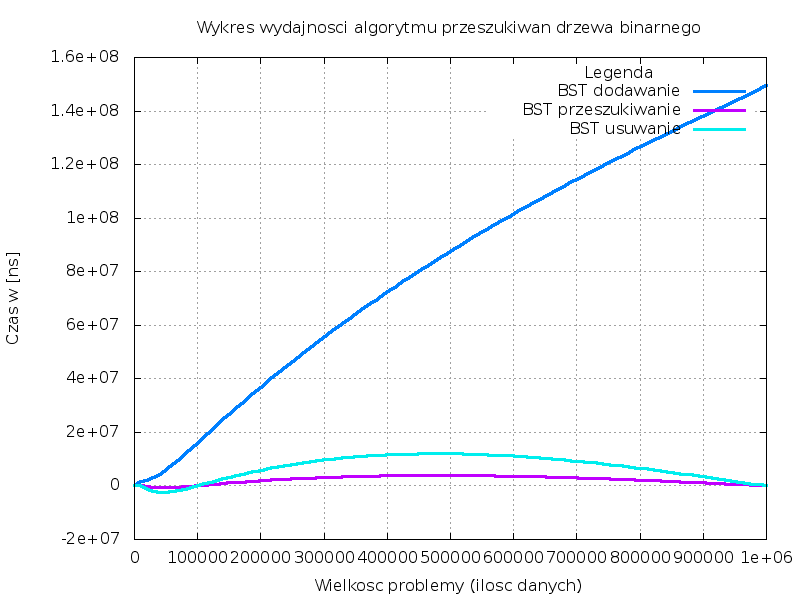
\includegraphics[scale = 0.4]{BST_result.png}
	\end{figure}
\end{center}

\newpage

\begin{table}[ht] 
\caption{Wyniki pomiarów dla tablicy haszującej} 
\centering 
\begin{tabular}{|c|c|c|c|}

\hline
\hline
Problem & Dodawanie [ns] & Szukanie [ns] & Usuwanie [ns]\\
\hline
10 & 88273.6 & 39855.7 & 29014.9 \\
\hline
100 & 172378 & 15925.4 & 19174.1 \\
\hline
1000 & 1.53564e+06 & 78268.7 & 77592 \\
\hline
10000 & 4.33938e+07 & 41062.5 & 11750 \\
\hline
100000 & 1.11948e+10 & 506938 & 16375 \\
\hline \hline

\end{tabular}
\end{table}

Poniżej dane zebrane w postaci wykresów.

\begin{center}
	\begin{figure}[h]
		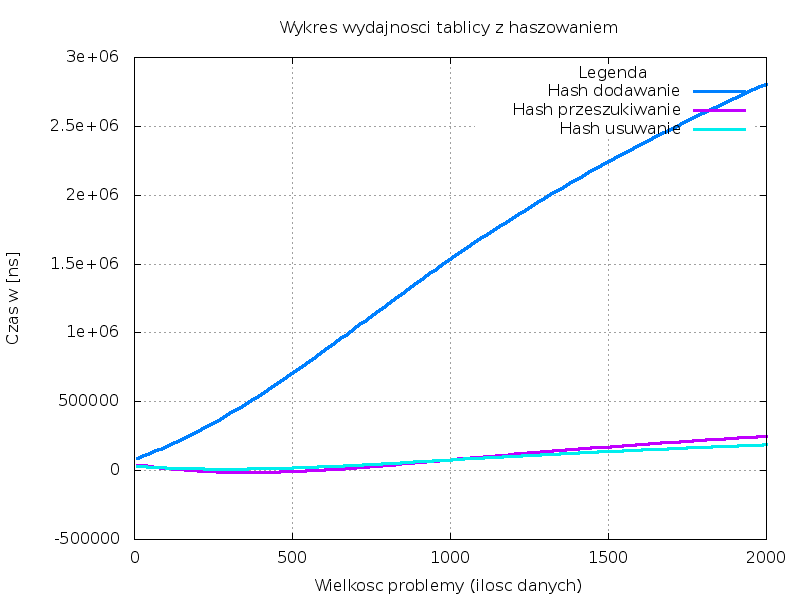
\includegraphics[scale = 0.4]{HSH_result.png}
	\end{figure}
\end{center}

\newpage

\section{Wnioski}

Tablica haszująca wydaje się być lepszą strukturą danych. Przemawiają za tym czasy wykonywania wszystkich trzech podjętych operacji. Duża rozbieżność pomiędzy czasami wykonywania operacji przez obie struktury oraz wynikające z nich kształty wykresów sugerują jednak błędną implementację tablicy haszującej. 
\end{document}



